\documentclass{book}

\usepackage[utf8]{inputenc}
\usepackage[T1]{fontenc}
\usepackage[portuguese]{babel}
\usepackage{ebgaramond}

\usepackage[paperheight   = 5.8in, % A6
            paperwidth    = 4.1in,
            bindingoffset = 0.2in,
            left          = 0.2in,
            right         = 0.3in,
            top           = 0.7in,
            bottom        = 0.6in,
            footskip      = 0.25in]{geometry}

\usepackage[labelformat = simple]{subfig}
\captionsetup[subfloat]{captionskip=10pt}
\renewcommand{\thesubfigure}{\relax} 

\usepackage{./goban/goban}

\def\sgfH{(
  ;GM[1]FF[4]CA[UTF-8]AP[Sabaki:0.52.2]KM[6.5]SZ[19]DT[2024-08-27]
  AW[pd]
  AB[od][pe][qd]
  ;B[pc]
)}

\begin{document}
  \begin{figure}[ht]
    \centering

    \subfloat[\large 1]{
      \begin{goban}[board dimension       = 8,
                    board size            = 19,
                    scale                 = 1,
                    outline line width    = 0.4mm,
                    horizontal clip start = 11,
                    horizontal clip end   = 19,
                    vertical clip start   = 11,
                    vertical clip end     = 19]
        \parseSgf{\sgfH}
      \end{goban}
    }

    \subfloat[\large 2]{
      \begin{goban}[board dimension       = 8,
                    board size            = 19,
                    scale                 = 1,
                    outline line width    = 0.4mm,
                    horizontal clip start = 11,
                    horizontal clip end   = 19,
                    vertical clip start   = 11,
                    vertical clip end     = 19]
        \parseSgf{\sgfH}
      \end{goban}
    }
  \end{figure}


  \begin{figure}
    \begin{minipage}[c]{0.5\linewidth}
      % 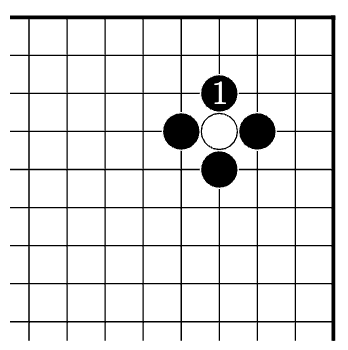
\includegraphics[width=\textwidth]{sgf/sgf_screenshot.png}
      \begin{goban}[board dimension       = 8,
                    board size            = 19,
                    scale                 = 1,
                    outline line width    = 0.4mm,
                    horizontal clip start = 11,
                    horizontal clip end   = 19,
                    vertical clip start   = 11,
                    vertical clip end     = 19]
        \parseSgf{\sgfH}
      \end{goban}

    \end{minipage}\hfill
    \begin{minipage}[c]{0.5\linewidth}
      \small A captura da pedra branca configura uma forma chamada \emph{ponnuki}, que é o número mínimo de pedras para se capturar uma pedra adversária, quando ela não está nem no canto e nem na borda. (Note que a pedra branca será retirada do tabuleiro.)
    \end{minipage}
  \end{figure}

  \begin{figure}
    \begin{minipage}[c]{0.5\textwidth}
      % 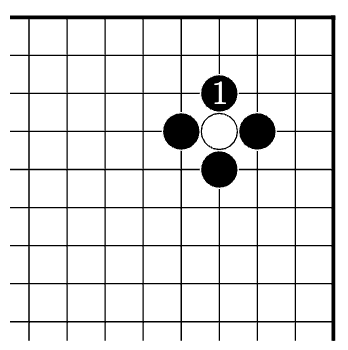
\includegraphics[width=\textwidth]{sgf/sgf_screenshot.png}
      \begin{goban}[board dimension       = 8,
                    board size            = 19,
                    scale                 = 1,
                    outline line width    = 0.4mm,
                    horizontal clip start = 11,
                    horizontal clip end   = 19,
                    vertical clip start   = 11,
                    vertical clip end     = 19]
        \parseSgf{\sgfH}
      \end{goban}

    \end{minipage}\hfill
    \begin{minipage}[c]{0.5\textwidth}
      \emph{Dia. 1.} Playing at 1 is great. Isn't it?
      % \caption{
      %   bakdfhjaldskjfla
      % }
    \end{minipage}
  \end{figure}
\end{document}